\documentclass[multi,crop=false,class=article]{standalone}

\begin{document}
\section{Tools and libraries}
\label{sec:tools}
The previous sections have shown that active automata learning is a currently 
studied computational learning process. However, as section 
\ref{sec:variants} has shown, there are some challenges in using active 
automata learning in a practical setting. To overcome these challenge as well 
as to promote active automata learning in practice, tools and libraries have 
been created. This section will give a brief overview of one library and one 
tool. This selection is based on the importance, availability and the amount of 
researches that have used those tools and libraries. First, the library 
Learnlib (\ref{ssec:learnlib}) will be discussed. Learnlib provides various 
active automata learning algorithms and optimizations. After that, the tool 
Tomte(\ref{ssec:tomte}) is discussed, which automatically generates 
abstractions for automata in order to apply active automata learning on them. 

\subsection{Learnlib}
\label{ssec:learnlib}

Learnlib\footnote{Supported through bug fixes and available from
\url{https://github.com/LearnLib/learnlib}} is a library that implements various
active learning algorithms as well as different configurations for learning
automata. It has been in development since 2009 \cite{Raffelt2009} and as of
2015, there has been a total overhaul of the library \cite{Isberner2015b}. To 
avoid confusion, the old version was renamed to JLearn.

The current version of this library consists out of two parts: Automatalib and
Learnlib.

\begin{figure}[!ht]
	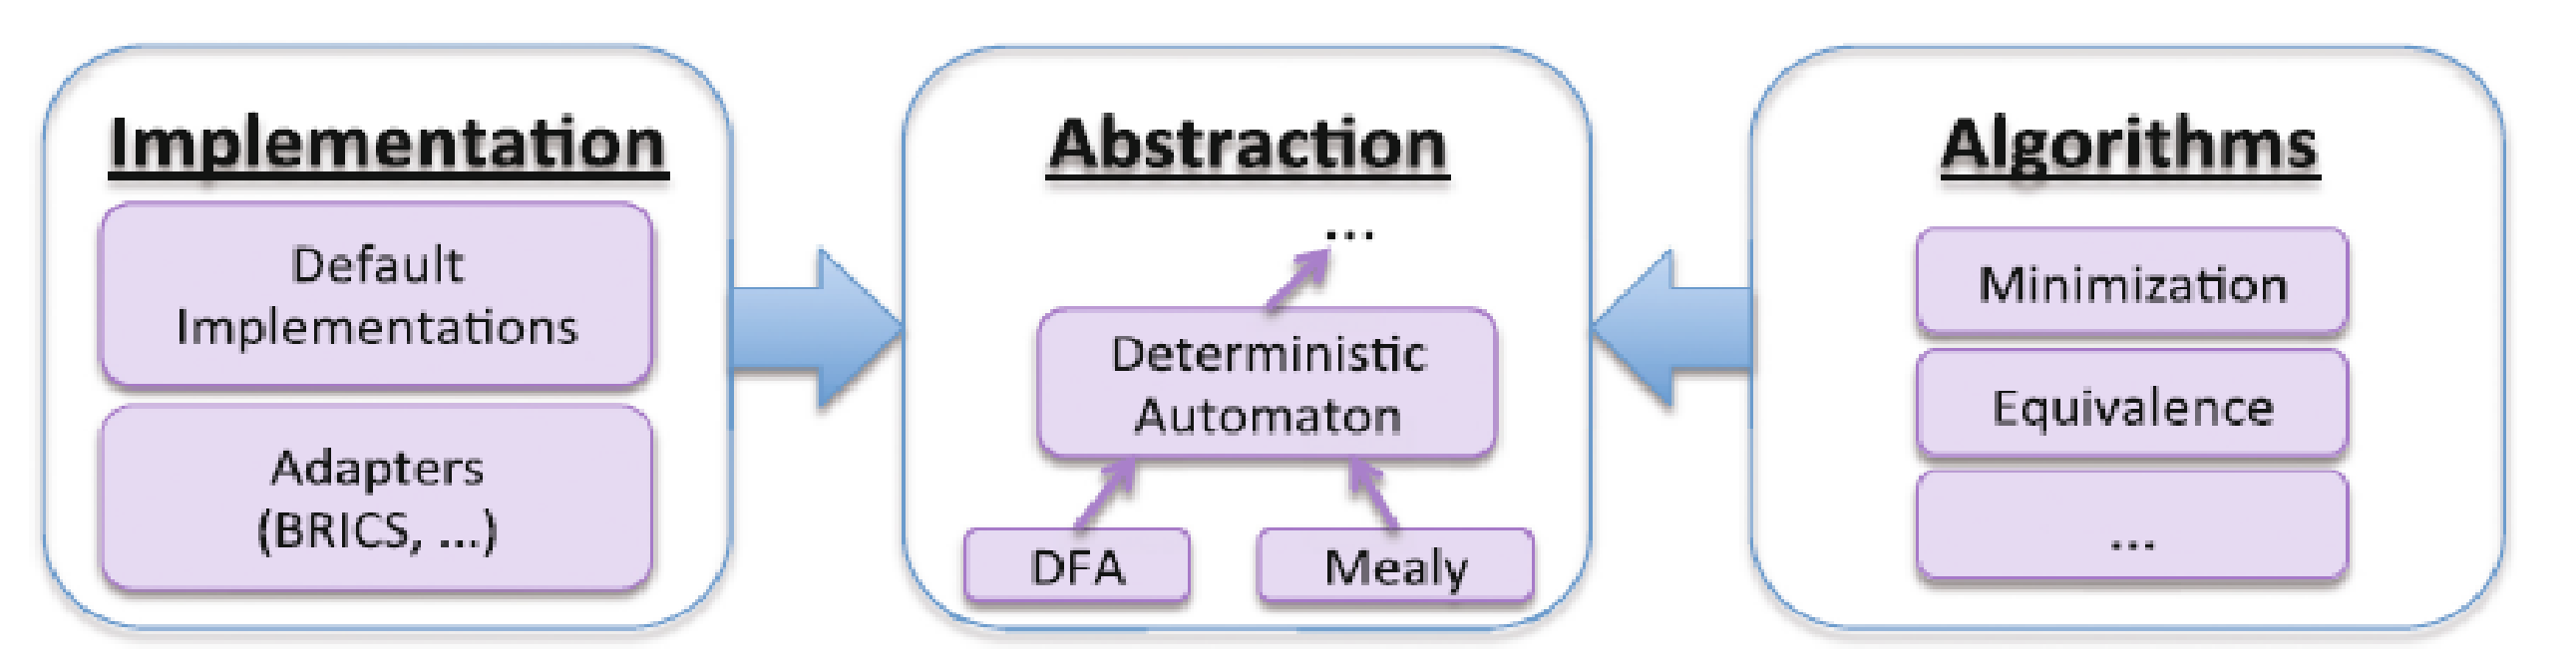
\includegraphics[width=\textwidth]{Tool_images/automatalib_architecture.png}
	\caption{Architecture of Automatalib, source is from \cite{Isberner2015b}}
	\label{fig:automatalib_arch}
\end{figure}

\paragraph{Automatalib} Automatalib is an independent library that contains 
abstract automata representations, automata data structures and algorithms (see 
figure \ref{fig:automatalib_arch}). The 
abstract automata representations make the library flexible because all data 
structures and algorithms depend on these representations. This makes it easy 
to add third party implementations of automata such as the BRICS library 
\cite{Alur2005}. Automatalib includes minimalization algorithms and equivalence 
testing algorithms based on Hopcroft and Karp's near-linear equivalence 
algorithm \cite{Hopcroft1971} or the W-Method (section \ref{sec:chow}) for 
black-box testing.

\begin{figure}[!ht]
	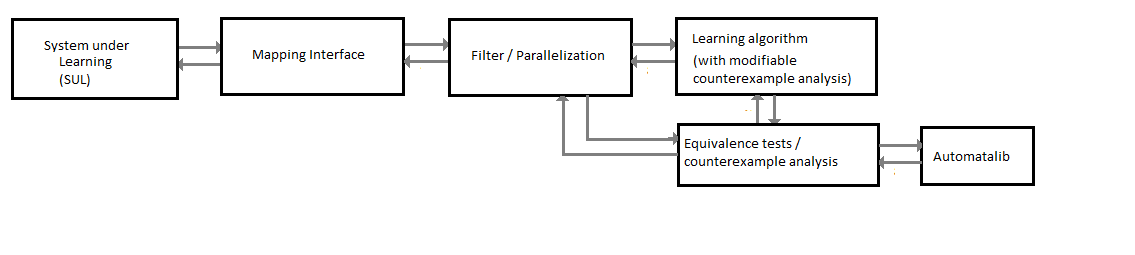
\includegraphics[width=\textwidth]{Tool_images/learnlib_architecture.png}
	\caption{Architecture of Learnlib}
	\label{fig:learnlib_arch}
\end{figure}

\paragraph{Learnlib} Learnlib is a library that provides learning algorithms and
infrastructure for automata learning. The learning algorithms consist of a base 
algorithm. This algorithm can be altered by replacing the counterexample 
analysis with other methods. All the official supported base algorithms with 
their alternative counterexample analysis are listed below:

\begin{itemize}
	\item L* (base) (see section \ref{ssec:AngluinLstar})
	\begin{itemize}
		\item Maler \& Pnueli's \cite{Maler1995}
		\item Rivest \& Schapnire's (see section \ref{sec:rivest-schap-count})
		\item Shahbaz's \cite{Shahbaz2009}
		\item Suffix1by1 \cite{Irfan2010}
	\end{itemize}
	\item Obversation Pack (base) \cite{Howar2012a}
	\item Kearns \& Vazirani's (base) (see section 
	\ref{sec:classification-trees})
	\item DHC (base) \cite{Merten2012}
	\item TTT (base) \todo{Reference to theory does not exists, yet}
	\item NL* (base) \cite{Bollig2009}
\end{itemize}

All the algorithms work with both DFAs and Mealy machines (see section 
\ref{sec:learn-mealy-mach}), except for DHC\cite{Merten2012} and 
NL*\cite{Bollig2009}.

For finding the counterexamples, Learnlib uses Automatalib as well as other
methods such as randomized tests. More methods can be found in 
\cite[p. 490]{Isberner2015b}.

Learnlib also offers filters that pre-process the queries of the learning 
algorithm. An example is the reduction of the amount of queries (see section 
\ref{sec:noreset}). Other examples are a mechanism for reducing the amount of 
resets  and a parallelization component that uses multiple teachers and 
parallel execution of membership queries\cite{Henrix2015,Howar2012}.     


\subsection{Tomte}
\label{ssec:tomte}
Tomte\footnote{In active development and available from
\url{http://tomte.cs.ru.nl/Tomte-0-4}} is a tool that automatically makes
abstractions for automata learning. It is essentially a translator between the
system under learning (SUL) and the learner. This makes tools such as Learnlib 
easier, since the user does not have to make the mapping manually.

\begin{figure}[!ht]
	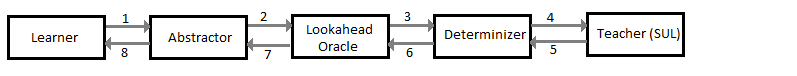
\includegraphics[width=\textwidth]{Tool_images/tomte_network.png}
	\caption{Architecture of Tomte}
	\label{fig:tomte_arch_interaction}
\end{figure}

The Abstractor, Lookahead Oracle and Determinizer together form Tomte. The
other two parts are not part of Tomte, but it comes with Learnlib for making 
the learner. The makers also have a tool\footnote{SUL tool available from 
\url{http://tomte.cs.ru.nl/Sut-0-4/Description}} available for creating the SUL 
since they must be modeled after a register automaton\cite{Aarts2015} 
(which is an extension of a Mealy machine).

\paragraph{Determinizer} The Determinizer elimates the nondeterministic
behaviour caused by the SUL. Since tools like Learnlib can only analyse
deterministic behaviour, it needs to converted. The theory behind it is
explained in \cite[p. 172]{Aarts2015}.

\paragraph{Lookahead Oracle} This oracle is used to annotate events of the SUL
with information about the impact on the future behaviour of the SUL. This way,
the Lookahead Oracle acts as a cache for the Abstractor. The theory and
implementation of this oracle is found in \cite[p. 170]{Aarts2014} and 
\cite[p. 105]{Tomte2014}.

\paragraph{Abstractor} The Abstractor is the component that creates the mapping
between the SUL and the learner. The idea behind the Abstractor is to make the 
model that needs to be learned by the Learner smaller than the SUL. This is 
needed, because a SUL typically has parameter values that make the alphabet 
large.

The Abstractor uses a concrete input set $\Sigma$ and a concrete 
output set $\Lambda$ used by the SUL. Then, with the help of  
counterexample-guided abstraction refinement\cite[p. 104]{Tomte2014} an 
abstracted input set $X$ and output set $Y$ is created. Those abstracted sets 
then represent a smaller model of the SUL. In order to make it scalable, this 
component also tries to reduce the length of the counterexample by removing 
loops and single transitions \cite{Koopman2014}. The complete theory is found 
in \cite{Tomte2014}.

\paragraph{Interaction between the modules} The exchange of messages between
all the modules is as follows (see numbering in figure
\ref{fig:tomte_arch_interaction}. For more information about this process see 
\cite{Aarts2015,Tomte2014}.

\begin{enumerate}
	\item The Learner sends an abstract query $x \in X$ to the Abstractor.
	\item The Abstractor receives an abstract query, selects a concrete input
	symbol $i \in \Sigma$ and sends it as a query to the Lookahead 
	Oracle. If no input symbol $i$ exists, return the symbol $\perp$ to the 
	Learner.
	\item The Lookahead Oracle checks if $i$ is cached. If not, then $i$ is send
	to the Determinizer. Otherwise, go to step 7.
	\item The Determinizer transforms the input back to the original behavior of
	the Teacher.
	\item The Determinizer receives the output from the Teacher and transforms 
	this into deterministic behavior.
	\item The Determinizer sends concrete symbol $o \in \Lambda$ to the 
	Lookahead Oracle which caches the pair $\{i,o\}$.
	\item The Lookahead Oracle sends $o$ together with the annotated information
	that came after the sequence of queries between the last reset query and
	$i$.
	\item Abstractor receives a concrete answer $o$ and the annotated
	information. It uses the annotated information to determine updates to the
	state variables of the Learner. It sends those updates and other
	information to the Learner as an abstract answer $y \in Y$.
\end{enumerate}

\end{document}

%%% Local Variables:
%%% mode: latex
%%% TeX-master: "main"
%%% End:
